\chapter{Design}
This design chapter provides a high-level overview of the software implementation. With the aid of visual tools such as diagrams, a plan for implementation will be outlined. 

\section{UML Sequence Diagram}
\hspace{0.5cm} A high-level overview from user input to output is important to illustrate so it may be followed in the latter sections of this chapter. Providing a visual representation also makes it easier to understand how all relevant components of the project interact from beginning to end. Most SPARQL Anything calls follow the same format as depicted in \textit{Figure 4} of \cite{asprino2023knowledge} and is strictly followed in \textit{Figure 7.1}. A contextualised UML Sequence diagram is shown in \textit{Figure 7.1}: 

\begin{figure}[H]
\begin{center}
    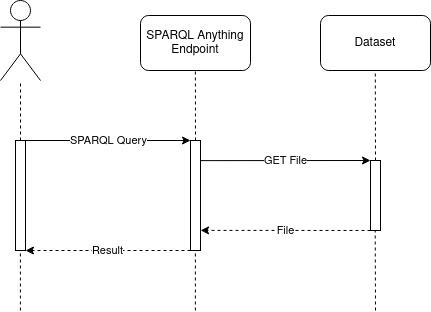
\includegraphics[width=8cm, height=6cm]{Images/UMLSequenceDiagram.drawio.png}
\end{center}
\vspace{-0.5cm}
\caption{UML Sequence Diagram}
\end{figure}
\vspace{-0.7cm}

\section{Ontology Structure}
\hspace{0.5cm} In this section, a plan for the ontology's general structure will be outlined based on: the dataset, provided ontology and any external websites. 

\begin{figure}[H]
    \begin{center}
        \begin{tikzpicture} [
            circle/.style={draw=blue, ellipse, ultra thick, fill=blue!30},
            align=center,
            node distance=2.5cm ]
            
        \node[circle] (q0) {Organ};
        \node[circle, right of=q0] (q1)  {Technical};
        \node[circle, left of=q0] (q2)  {Changes};
        \node[circle, above of=q0] (q3)  {Disposition};
        \node[circle, below of=q0] (q4)  {OrganWikidata};
    
        \draw[] (q0.east) -- (q1.west);
        \draw[] (q0.west) -- (q2.east);
        \draw[] (q0.north) -- (q3.south);
        \draw[] (q0.south) -- (q4.north);
            
        \end{tikzpicture}
    \end{center}
    \vspace{-0.4cm}
\caption{Core Organ Ontology}
\end{figure}
\vspace{-0.1cm}

\textit{Figure 7.2} illustrates the main components to be expanded on in the ontology based on data in the dataset. More details of the main nodes are detailed below:

\begin{enumerate}
    \item \textbf{Organ}: The primary organ component that will connect with other many other nodes.
    \item \textbf{Changes}: This component specifies the organ adjustment details and maintenance changes for an organ.
    \item \textbf{Disposition}: This component refers to the organ's current components and details relating to them.
    \item \textbf{Technicals:} This component is responsible for the specific musical details of the organ. 
    \item \textbf{OrganWikidata}: This provides an expansion of the existing knowledge graph from Wikidata.
\end{enumerate}

The section of the ontology specifically for external Wikidata links can be structured in the same format as displayed on its website. Using \textit{Figure 7.2}, extending the \textit{OrganWikidata} node is most plausible. For instance, the organ page on Wikidata \cite{organwikidata} contains organ-related triples. An extract from \cite{organwikidata} is shown below:

\lstset
{
    breaklines=true,
    breakatwhitespace=true,
    basicstyle=\linespread{1.5}\ttfamily,
}
\begin{lstlisting}
organ subclassOf keyboardInstrument
organ subclassOf buildingComponent
organ studiedBy organology 
...
\end{lstlisting}

In this case, `organ' can be replaced with our \textit{OrganWikidata} node and the corresponding relationships and objects will be added to the ontology. All the extra nodes and edges can be added as external links to the knowledge graph using their unique Wikidata URI. 

\section{Query Flow Diagram}
\hspace{0.5cm} A flow diagram is a graphical representation of the sequence of steps or actions that need to be taken to complete a process. \cite{flowchart}

In this section, the logic required to build the SPARQL Anything Query will be illustrated in the form of a flow diagram. This will provide the structure required to build the query and produce a knowledge graph.

\begin{figure}[H]
    \begin{center}
        \begin{tikzpicture} [
            circle/.style={draw=green, ellipse, ultra thick, fill=green!30},
            align=center,
            node distance=2.5cm ]
        \node[circle] (q0) {1. Add ontology};
        \node[circle, below of=q0] (q1)  {2. Query dataset};
        \node[circle, below of=q1] (q2)  {3. Clean \& create data path};
        \node[circle, below of=q2] (q3)  {4. Retrieve data from dataset};
        \node[circle, below of=q3] (q4)  {5. Add to Knowledge Graph};
        \node[circle, below of=q4] (q5)  {6. Clean \& create external link};
        \node[circle, below of=q5] (q6)  {7. Add to Knowledge Graph};
        \node[circle, below of=q6] (q7)  {8. Add any other external links};
        \node[circle, below of=q7] (q8)  {9. Output Knowledge Graph};
    
        \draw[->] (q0.south) -- (q1.north);
        \draw[->] (q1.south) -- (q2.north);
        \draw[->] (q2.south) -- (q3.north) node [midway, fill=white] {Using cleaned data};
        \draw[->] (q3.south) -- (q4.north);
        \draw[->] (q4.south) -- (q5.north);
        \draw[->] (q5.south) -- (q6.north);
        \draw[->] (q6.south) -- (q7.north);
        \draw[->] (q7.south) -- (q8.north);
        \draw[->] (q4.east) to [out=0,in=0] (q2.east);
        \draw[->] (q4.east) to [out=0,in=0] (q7.east);
        \draw[->] (q6.west) to [out=180,in=180] (q2.west);
    
        \end{tikzpicture}
    \end{center}
    \vspace{-0.4cm}
    \caption{Query Flow Diagram}
\end{figure}
\vspace{-0.1cm}

The nodes in \textit{Figure 7.3} represent necessary actions and one of the edges is explicitly stated so that the process is clear. Below, an explanation for each node is provided: 

\begin{enumerate}
  \item \textbf{`Add ontology' node} \\ Adds ontology to the \textit{CONSTRUCT} clause of the query.
  \item \textbf{`Query dataset' node} \\ Uses SPARQL Anything to specify the file containing data of interest.
  \item \textbf{`Clean \& create data path' node} \\ Uses string manipulation in order to create a valid path to desired data in the dataset. 
  \item \textbf{`Retrieve data from dataset' node} \\ Uses created path above to retrieve correct data.
  \item \textbf{`Add to knowledge graph' node} \\ Adds retrieved data to the knowledge graph. Then, it either loops to step 3 using a different JSON file, continues to step 6 by adding custom external links or skips to step 8 to add other independent external links. The latter pertains to the last SPARQL Anything call in the query. 
  \item \textbf{`Create \& clean external link' node} \\ Creates an external link using retrieved data within the same SPARQL Anything call.
  \item \textbf{`Add to knowledge graph' node} \\ Adds the custom external link to the knowledge graph. Then, it either loops to step 3 using a different JSON file or skips to step 8 to add other independent external links. The latter pertains to the last SPARQL Anything call in the query. 
  \item \textbf{`Add any other external links' node} \\ Adds any other links that do not require data from the dataset such as Wikidata and MusicBrainz.
  \item \textbf{`Output knowledge graph' node} \\ Produces the resulting knowledge graph.
\end{enumerate}

\section{Query Skeleton Structure}
\hspace{0.5cm} In this section, the flow diagram, illustrated in \textit{section 7.3}, will be used to structure the query. 

\lstset
{
    breaklines=true,
    breakatwhitespace=true,
    basicstyle=\linespread{1.25}\ttfamily,
}
\begin{lstlisting} 
PREFIX ... # Add relevant links

CONSTRUCT {
    ... # Add organ ontology
} 
WHERE 
    { 
        SERVICE <x-sparql-anything:file:./___.json>  # Query dataset
        { 
            ... # Clean and create data path
            ... # Retrieve data from dataset
            ... # Add to Knowledge Graph
            ... # Clean and create external link (if applicable)
            ... # Add to Knowledge Graph
        } 
        SERVICE <x-sparql-anything:file:./___`.json>  # Query dataset
        { 
            ... # Clean and create data path
            ... # Retrieve data from dataset
            ... # Add to Knowledge Graph
            ... # Clean and create external link (if applicable)
            ... # Add to Knowledge Graph
        } 
        .
        .
        .
        ... # Add any other external links 
        # Output Knowledge Graph
    }
}
\end{lstlisting}

This basic query structure follows all steps in \textit{Figure 7.3} and aids query creation to generate a knowledge graph. This can be observed in the comments next to each line, which correspond to a step in the flow diagram created. It also outlines the basic structure that will be used to create the query. The multiple SERVICE calls specify the  JSON file in the dataset being queried. 

